\documentclass[12pt]{beamer}

\usepackage[utf8]{inputenc}
\usepackage[T1]{fontenc}
\usepackage[croatian]{babel}

\usepackage{algorithm}
\usepackage{algpseudocode}

\usetheme{metropolis}           % Use metropolis theme

\title{Raymarching}
\date{10. siječnja 2019.}
\author{Nikola Bunjevac}
\institute{Fakultet elektrotehnike i računarstva}

\begin{document}
  \maketitle

  \begin{frame}{Sadržaj}
    \tableofcontents
  \end{frame}

  \section{Uvod}

  \begin{frame}{Uvod}
    \begin{itemize}
    \item GPU
    \item Sjenčar (engl. {\sl shader}\/)
    \item Izvođenje u stvarnom vremenu
    \item Eksploatacija paralelizma
    \end{itemize}
  \end{frame}

  \section{Algoritam Raymarching}

  \begin{frame}{Algoritam}
    \begin{itemize}
    \item Aproksimacijski algoritam (za razliku od raytracinga)
    \item Konačan broj koraka
    \item Izvodi se u sjenčaru fragmenata
      \begin{itemize}
      \item Poligon (pravokutnik) prikazan preko cijelog ekrana
      \item Imamo pristup svakom pikselu prozora (UV koordinate)
      \item Uniformne varijable
      \end{itemize}
    \item Prilično jednostavan
    \item Moguća interaktivnost
    \end{itemize}
  \end{frame}

  \begin{frame}{Pseudokod}
    \begin{algorithm}[H]
      \floatname{algorithm}{Algoritam}
      \caption{Funkcija Raymarch}
      \begin{algorithmic}[1]
        \Function{Raymarch}{vec3 $ro$, vec3 $rd$}
          \State float d = 0.0;
          \For{(int i = 0; i < \texttt{MAX\_STEPS}; i++)}
            \State vec3 p = ro + d*rd;
            \State float dS = \Call{getDist}{p}; // funkcija udaljenosti
            \State d += dS;
            \If{(dS < \texttt{SURFACE\_DIST} || d > \texttt{MAX\_DIST})}
              \State break;
            \EndIf
          \EndFor
          \State \Return d;
        \EndFunction
      \end{algorithmic}
      \label{alg:raymarch}
    \end{algorithm}
  \end{frame}

  \begin{frame}{Ilustracija}
    \begin{figure}
      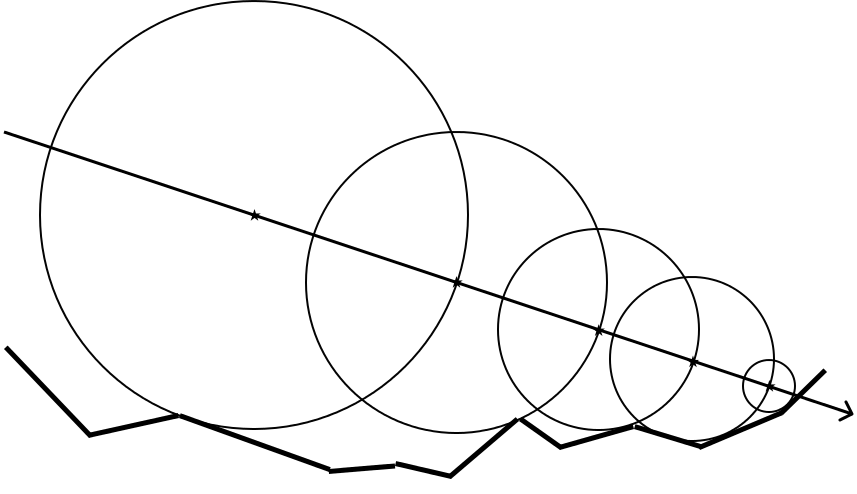
\includegraphics[width=\textwidth,height=\textheight,keepaspectratio]{raymarch.png}
      \caption{Raymarching (izvor: http://digitalfreepen.com)}
    \end{figure}
  \end{frame}

  \begin{frame}{Funkcija udaljenosti}
    \begin{itemize}
    \item Objekti se modeliraju matematičkim funkcijama
    \item Prilično moćno, ali nezgrapno
    \item Moguće kombinirati razne funkcije
          \begin{itemize}
          \item Zbrajanje
          \item Oduzimanje
          \item Odmak/izobličenje (engl. {\sl displacement}\/)
          \item Zaobljivanje
          \item Uvrtanje
          \item Transformacije
          \end{itemize}
        \item \href{https://www.iquilezles.org/www/articles/distfunctions/distfunctions.htm}{https://www.iquilezles.org/www/articles/
                 distfunctions/distfunctions.htm}
    \end{itemize}
  \end{frame}

  \section{Primjeri}

  \begin{frame}{Demonstracija}
    \begin{itemize}
    \item Jednostavna scena
      \begin{itemize}
        \item \texttt{./raymarching shader.frag}
      \end{itemize}
    \item Puno objekata + boje
      \begin{itemize}
        \item \texttt{./raymarching cubes.frag}
      \end{itemize}
    \item Puno objekata drugog oblika
      \begin{itemize}
        \item \texttt{./raymarching tori.frag}
      \end{itemize}
    \item Kompleksni oblik
      \begin{itemize}
        \item \texttt{./raymarching complex.frag}
      \end{itemize}
    \end{itemize}

    Program je isti, samo se sjenčar fragmenata mijenja!
  \end{frame}

  \begin{frame}{Još puno mogućnosti}
    \begin{figure}
      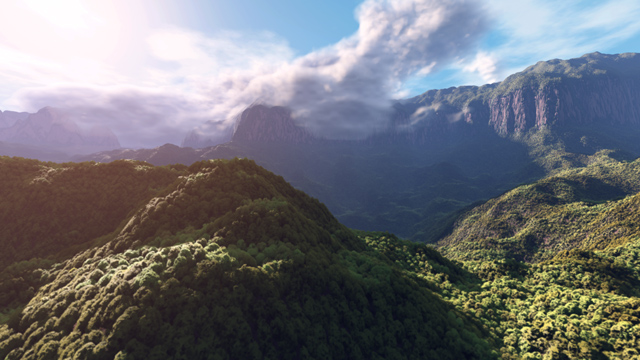
\includegraphics[width=\textwidth,height=\textheight,keepaspectratio]{rainforest.jpg}
      \caption{Prašuma (autor: Íñigo Quílez)}
    \end{figure}
  \end{frame}

    \begin{frame}{Još puno mogućnosti}
    \begin{figure}
      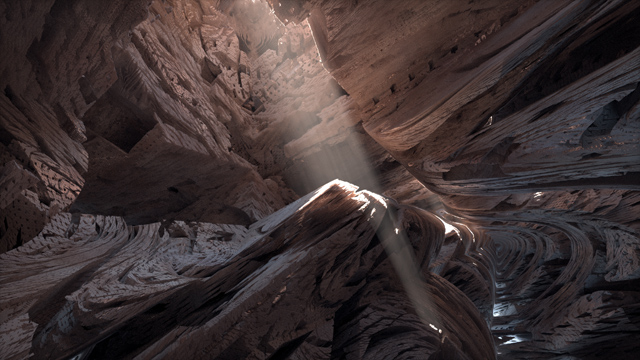
\includegraphics[width=\textwidth,height=\textheight,keepaspectratio]{sponge.jpg}
      \caption{Spužva (autor: Íñigo Quílez)}
    \end{figure}
    Izvor: \href{https://www.iquilezles.org/www/articles/raymarchingdf/raymarchingdf.htm}{https://www.iquilezles.org/www/articles/raymarchingdf/raymarchingdf.htm}{Íñigo Quílez}
  \end{frame}

  \begin{frame}{Nedostaci}
    \begin{itemize}
    \item Ograničenost sjenčara
    \item Definiranje objekata/modela
    \item Aproksimacija
    \item Teksture (UV koordinate, problemi s rubovima)
    \end{itemize}
  \end{frame}

  \begin{frame}{Literatura}
    \begin{itemize}
    \item \href{https://www.youtube.com/watch?v=PGtv-dBi2wE}{https://www.youtube.com/watch?v=PGtv-dBi2wE} (Ray Marching for Dummies!)
    \item \href{https://www.iquilezles.org/www/}{https://www.iquilezles.org/www/}
    \item \href{http://jamie-wong.com/2016/07/15/ray-marching-signed-distance-functions/}{http://jamie-wong.com/2016/07/15/ray-marching-signed-distance-functions/}
    \end{itemize}
  \end{frame}

\end{document}
